\documentclass[conference]{IEEEtran}
\IEEEoverridecommandlockouts
% The preceding line is only needed to identify funding in the first footnote. If that is unneeded, please comment it out.

\usepackage{amsmath,amssymb,amsfonts}
\usepackage{algorithmic}
\usepackage{graphicx}
\usepackage{textcomp}
\usepackage{xcolor}
\def\BibTeX{{\rm B\kern-.05em{\sc i\kern-.025em b}\kern-.08em
    T\kern-.1667em\lower.7ex\hbox{E}\kern-.125emX}}

\usepackage[style=ieee,doi=false,maxbibnames=3]{biblatex}
\addbibresource{references.bib}


\begin{document}

\title{Caching in Named Data Networking for the Wireless Internet of Things}

\author{\IEEEauthorblockN{Merlin Steuer}
\IEEEauthorblockA{Universität zu Lübeck}\\
Lübeck, Germany \\
merlin.steuer@student.uni-luebeck.de
}

\maketitle

\begin{abstract}
Named Data Networking (NDN) is a promising approach for Internet of Things (IoT) networks thanks to innovative approaches like name-based routing and in-network caching. This paper proposes a novel probabilistic caching strategy that is well-suited for wireless IoT applications. By simulating an NDN network we find the new strategy to be beneficial on both energy consumption and data response times.
\end{abstract}

%\begin{IEEEkeywords}
%    Named Data Networking, Information-Centric
%    Networking, Internet of Things, In-network caching, Freshness
%\end{IEEEkeywords}

\section{Introduction}

In recent years, the Internet of Things (IoT) has become increasingly important and the variety of connected devices is steadily rising, ranging from tiny sensors and actuators to big and powerful smartphones or even vehicles. In addition to that, the kind of data exchanged in these networks has also changed from big, static documents to small, transient data, for example, sensor readings produced by such devices.

The researchers in \cite{Hail2015} focused on wireless devices, which usually have limited energy resources and small memory sizes, creating a need for efficient communication (thus reducing the number of radio transmissions) and memory usage.

The researchers propose a new caching strategy for Named Data Networks, {pCASTING} (\textit{probabilistic {CAching} STrategy for the {INternet} of {thinGs}}), which is especially suited for applications in wireless IoT networks. It could be shown that the strategy is beneficial for both energy consumption and memory usage while also increasing data availability and decreasing response times to data requests.

The content of this short paper is as follows. In section \ref{sec:background} a short introduction to Named Data Networking and caching strategies is given. In Section~\ref{sec:pcasting} the proposed caching strategy is discussed in detail. In Section~\ref{sec:eval} the strategy is evaluated and the paper is concluded in Section~\ref{sec:conclusion}.

\section{Background}
\label{sec:background}

\subsection{Named Data Networking}

NDN is a content dissemination architecture for the future internet. It employs hierarchical URI-like content names which are carried in so-called \textit{Interest} and \textit{Data} packages. As opposed to current content delivery technologies, NDN can be employed as a protocol directly above the link layer\cite{Baccelli2014}, reducing the communication overhead and thus energy efficiency in wireless applications.

Each NDN node consists of the following data tables:
    \textit{(i)} The content store (CS) which is used to cache incoming data,
    \textit{(ii)} the Pending Interest Table (PIT) in which pending data requests are stored and
    \textit{(iii)} the Forwarding Information Base (FIB), used as a routing table, deciding on routes based on content names.

When an \textit{Interest} arrives at a node, it first checks whether there is already data with the given content name in the CS. If this is the case, the data is returned to the requesting node. Otherwise, the node checks whether there already is a pending Interest in the PIT matching the content name. If there already exists an entry in the PIT, the Interest is discarded. If no such entry exists, the Interest is forwarded using the routing information in the FIB. When the Data packet returns to a node, it forwards the data packet to all corresponding nodes stored in the PIT. Each node may decide to cache the data in the CS for further requests of the same content name.

\subsection{Caching in Named Data Networking}

The caching system in an NDN node consists of two components: (i) the caching strategy, deciding whether incoming data should be cached, and (ii) a replacement policy, deciding which data in the cache shall be dropped when the CS is full.

Many different caching strategies have been proposed, including probabilistic caching\cite{Tarnoi2014}. The key idea behind this approach is that a node caches data based on a probability $p$ with $0 \leq p \leq 1$. The \textit{Cache Everything Everywhere (CEE²)} strategy is a special case of probabilistic caching with $p = 1$. Lowering $p$ decreases the chance of data being cached while increasing the diversity of cached data in the overall network.

In IoT networks, the classic caching approaches reach their limits due to the limited memory space and transient data. The research in \cite{Baccelli2014} shows however that caching still has a beneficial impact on these networks, as it can drastically reduce the number of radio transmissions needed within a network.

\section{The pCASTING Caching Strategy}
\label{sec:pcasting}

The caching strategy introduced in the research targets \textit{simplicity} and \textit{no overhead}. The pCASTING caching strategy is executed on each node completely independently. Additionally, pCASTING is independent of the used routing protocol\cite{Amadeo2014}. As a first step, pCASTING calculates the probability at which data is cached in a node. As a second step, the node decides whether to cache data using the previously calculated probability.

The researchers describe attributes connected to the device or the data which are taken into account when calculating the caching probability. Namely:
\begin{enumerate}
	\item The device's energy level $EN$ with $0 \leq EN \leq 1$.
	\item The device's current cache occupancy $OC$ with $0 \leq OC \leq 1$. A value of $0$ means that the cache is empty, $1$ represents a full cache respectively.
	\item The residual freshness $FR = 1 - \frac{currentTime - t_s}{f}$ with $t_s$ being the timestamp at which the data was sampled and $f$ indicating for how long a datum is valid.
\end{enumerate}

These three parameters are then combined to calculate a caching probability $F_u$ at a given node.
\begin{equation}
	F_u = \sum_{i = 1}^{N_p} w_i g(x_i)
\end{equation}

where the $x_i$ describe the values $OC$, $EN$, and $FR$. The weights $w_i$ are chosen such that $0 \leq w_i \leq 1$ and $\sum_{i = 1}^{N} w_i = 1$. The utility function $g(x_i)$ is defined as the power function $g(x_i) = x_i^n$, $n \geq 1$, thus ensuring monotony in the interval of $[0; 1]$ and putting more impact on values that are near to the limits of the interval. The final function $F_u$ for the above parameters then is defined as the weighted sum of power functions:
\begin{equation}
	F_u = w_1 \cdot EN^n + w_2 \cdot (1 - OC)^n + w_3 \cdot FR^n
\end{equation}

$F_u$ is calculated by every node upon arrival of every Data packet.

\section{Evaluation}
\label{sec:eval}

To evaluate the effectiveness of {pCASTING} in terms of energy consumption and data retrieval times, simulations were performed in the simulation tool {ndnSIM}. A set of 60 mobile forwarding nodes were simulated, as well as a set of fixed Access Point (AP) and sensor nodes. In all nodes, the energy level was simulated to fall while communicating. During the experiments, {pCASTING} was compared to three other caching strategies: \textit{(i)} Cache Everything Everywhere (CE²), \textit{(ii)} No caching and \textit{(iii)} $P(0.5)$, where the probability of a data packet being cached is fixed to $0.5$.

Two main experiments were performed: A \textit{Network Lifetime Analysis} to analyze whether the caching strategy would impact the overall energy consumption and thus network lifetime, as well as a \textit{Retrieval Performance Analysis}.

The results of the first experiment are shown in Figure \ref{fig}. With the {pCASTING} strategy applied, the nodes in the wireless network were operational for a longer amount of time, indicating that {pCASTING} has a beneficial effect on energy usage by reducing the amount of radio communications.

Additionally, Table \ref{tab} displays the simulation results of the second experiment, giving the simulated cache hit ratio and the data retrieval time for the different caching approaches. The experiments have shown that {pCASTING} offers a higher data availability in caches while also allowing nodes to respond quicker than when the other (or no) caching strategies are applied.

\begin{figure}
	\begin{center}
	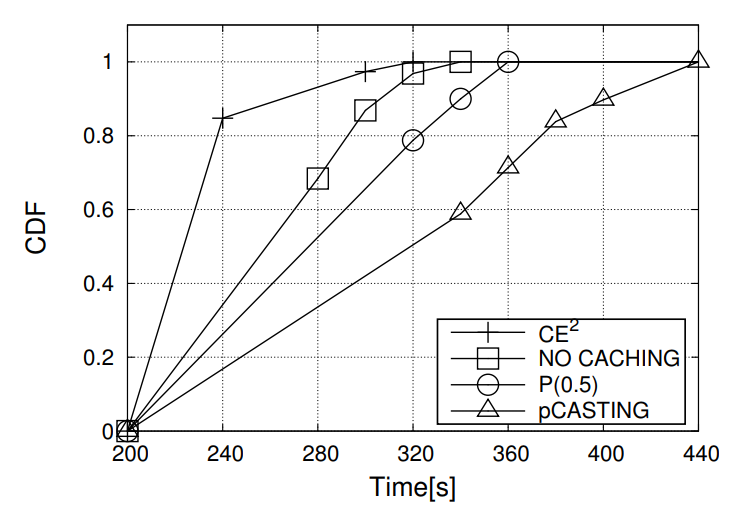
\includegraphics[width=0.3\textwidth]{fig1.png}
	\end{center}

	\caption{Cumulative Distribution Function of the discharge time of the nodes in the network.}
	\label{fig}
\end{figure}

\begin{table}
	\begin{center}
		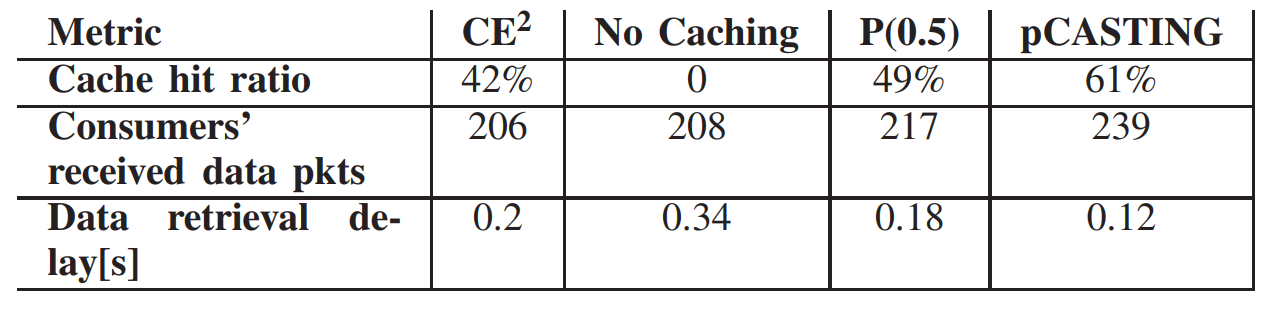
\includegraphics[width=0.4\textwidth]{tab1.png}
	\end{center}
	\caption{Data dissemination performance metrics for the different caching strategies.}
	\label{tab}
\end{table}

\section{Conclusion}
\label{sec:conclusion}

In this paper, the {pCASTING} caching strategy was proposed for in-network caching in wireless IoT applications. The strategy adjusts the caching probability according to three main attributes of a device: Its energy level, cache occupancy, and data freshness. It could be shown in simulations, that the strategy can reduce energy consumption in the nodes while at the same time reducing content retrieval delays. The {pCASTING} caching strategy can be easily extended by adding new attributes to the probability computation, providing a good basis for future work.

\printbibliography

\end{document}
